
\section{Signal processing for vibration analysis}
Vibration data is vital for health assessment of a given system and carries out very useful information about its performance (refer to section \ref{sec:data-acquisition} for details about data acquisition), yet these information are usually hard to observe in its raw waveform. Signal processing techniques are used to convert the raw waveform from time domain into frequency or time–frequnecy domains.

\section{Fourier analysis}
Fourier analysis, also called harmonic analysis, of a periodic signal $x(t)$ is the decomposition of the series into summation of sinusoidal components, where each sinusoid has a specific amplitude and phase.

The Fourier transform (FT) of a signal $x(t)$ can be mathematically given by equation \ref{equation:fourier-transform}:

\begin{equation}
    X(w) = \int_{-\infty}^{\infty}x(n)e^{-jwt}dt
    \label{equation:fourier-transform}
\end{equation}

In practical applications of digital signal processing where signals are discrete in time rather than continuous (e.g. vibration analysis) a discretized version called discrete fourier transform (DFT) is used instead, it is expressed mathematically by equation \ref{equation:discrete-fourier-transform}:

\begin{equation}
    X(w) = \sum_{-\infty}^{\infty}x(t)e^{-jwt}dt
    \label{equation:discrete-fourier-transform}
\end{equation}

Fast Fourier transform (FFT) is an effective algorithm used to implement DFT in computers. Figure \ref{figure:fft} shows a signal in its waveform (or time domain) and its corresponding spectrum (frequency domain) obtained using FFT algorithm. The spectrum shows the frequency components present in the signal:

\begin{figure}[H]
    \centering
    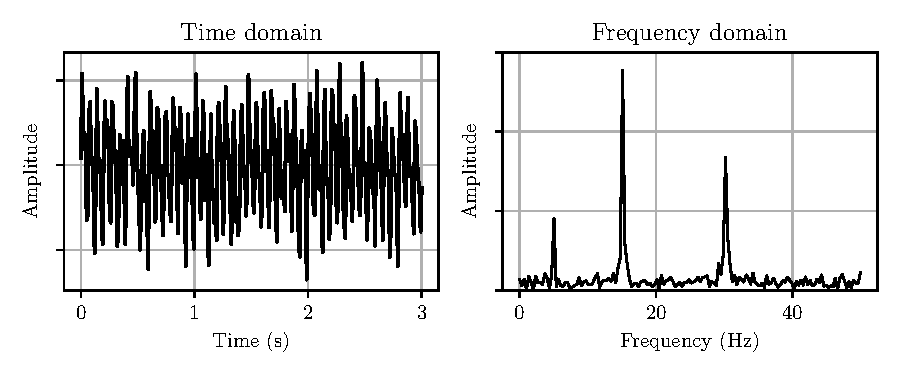
\includegraphics{figures/fft.pdf}
    \caption{Signal in the time domain and its fast Fourier transform}
    \label{figure:fft}
\end{figure}

\section{Wavelet transform}
Wavelet transform is also a spectral analysis tool, like Fourier transform. The main difference is that Fourier transform decomposes the signal into sinusoidal components, but wavelet transform decomposes it into a set of oscillatory functions called \textbf{wavelets}. Unlike sinusoids, wavelets are localized in time, thus wavelet transform doesn't only provide information about the frequency present in a signal but also the time of their occurence. Wavelet transform is a much better solution than Fourier transform when studying non-linear non-stationary signals (i.e. its frequency components vary with time).

Figure \ref{fig:time-frequency-plane} shows the difference in time and frequency resolutions between different methods. In the waveform, the signal has absolute resolution in time and zero resolution in frequency. Fourier transform on the contrary transforms the signal totally into the frequency domain, therefore it has absolute resolution in frequency but no resolution in time. Short-time Fourier transform is calculated identically to fourier transform but it is performed on separate segments of the original signal to preserve some resolution in time. Wavelet transform on the other hand exhibits a high time resolution for high frequencies and high frequency resolution for low frequencies:

\begin{figure}[H]
    \centering
    \begin{subfigure}{.35\textwidth}
	\centering
	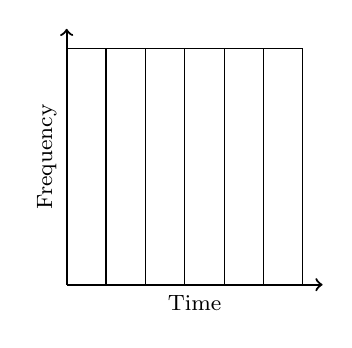
\begin{tikzpicture}
	\draw (0,0) -- (3,0);
	\draw (3,0) -- (3,-3);
	\path[thick, ->]  (0,-3) edge node[below] {\footnotesize Time} (3.25,-3)  ;
	\path[thick, ->] (0,-3) edge node[above, rotate=90] {\footnotesize Frequency} (0,.25)  ;
	
	\draw (.5,0) -- (.5,-3);
	\draw (1,0) -- (1,-3);
	\draw (1.5,0) -- (1.5,-3);
	\draw (2,0) -- (2,-3);
	\draw (2.5,0) -- (2.5,-3);
	
	\draw (3,0) -- (3,-3);
	\end{tikzpicture}
	\caption{Waveform}
\end{subfigure}%
\begin{subfigure}{.35\textwidth}
	\centering
	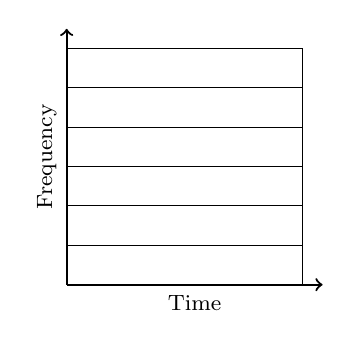
\begin{tikzpicture}
	\draw (0,0) -- (3,0);
	\draw (3,0) -- (3,-3);
	\path[thick, ->]  (0,-3) edge node[below] {\footnotesize Time} (3.25,-3)  ;
	\path[thick, ->] (0,-3) edge node[above, rotate=90] {\footnotesize Frequency} (0,.25)  ;
	
	\draw (0,-.5) -- (3,-.5);
	\draw (0,-1) -- (3,-1);
	\draw (0,-1.5) -- (3,-1.5);
	\draw (0,-2) -- (3,-2);
	\draw (0,-2.5) -- (3,-2.5);
	
	\end{tikzpicture}
	\caption{Fourier Transform}
\end{subfigure}

\medskip

\begin{subfigure}{.35\textwidth}
	\centering
	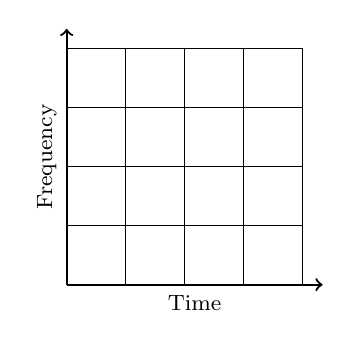
\begin{tikzpicture}
	
	\draw (0,0) -- (3,0);
	\draw (3,0) -- (3,-3);
	\path[thick, ->]  (0,-3) edge node[below] {\footnotesize Time} (3.25,-3)  ;
	\path[thick, ->] (0,-3) edge node[above, rotate=90] {\footnotesize Frequency} (0,.25)  ;
	
	\draw (0.75,0) -- (0.75,-3);
	\draw (0,-0.75) -- (3,-0.75);
	\draw (1.5,0) -- (1.5,-3);
	\draw (2.25,0) -- (2.25,-3);
	\draw (0,-1.5) -- (3,-1.5);
	%	\draw (3,0) -- (3,-3);
	\draw (0,-2.25) -- (3,-2.25);
	
	\end{tikzpicture}
	\caption{Short-Time Fourier}
\end{subfigure}%
\begin{subfigure}{.35\textwidth}
	\centering
	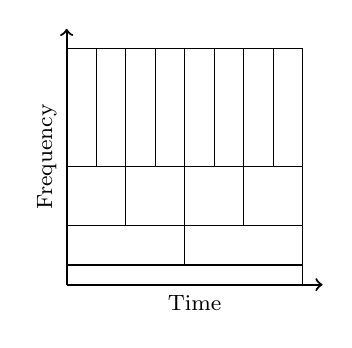
\begin{tikzpicture}
	\draw (0,0) -- (3,0);
	\draw (3,0) -- (3,-3);
	\path[thick, ->]  (0,-3) edge node[below] {\footnotesize Time} (3.25,-3)  ;
	\path[thick, ->] (0,-3) edge node[above, rotate=90] {\footnotesize Frequency} (0,.25)  ;
	\draw (0,-1.5) -- (3,-1.5);
	\draw (0,-2.25) -- (3,-2.25);
	
	\draw (0,-2.75) -- (3,-2.75);
	\draw (1.5,0) -- (1.5,-2.75);
	
	\draw (0.75,0) -- (0.75,-2.25);
	\draw (2.25,0) -- (2.25,-2.25);
	
	\draw (0.375,0) -- (0.375,-1.5);
	\draw (1.125,0) -- (1.125,-1.5);
	\draw (1.875,0) -- (1.875,-1.5);
	\draw (2.625,0) -- (2.625,-1.5);
	\end{tikzpicture}
	\caption{Wavelet Transform}
\end{subfigure}


\begin{comment}
%BIGGER VERSION

\begin{subfigure}{.4\textwidth}
	\centering
	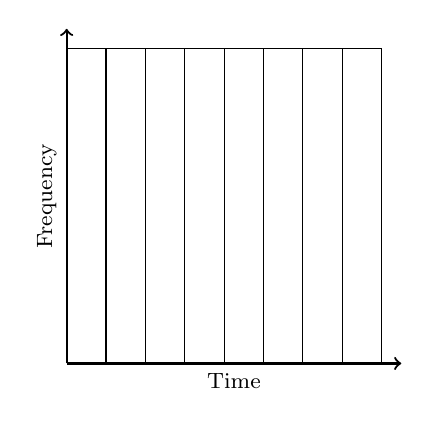
\begin{tikzpicture}
	\draw (0,0) -- (4,0);
	\draw (4,0) -- (4,-4);
	\path[thick, ->]  (0,-4) edge node[below] {\footnotesize Time} (4.25,-4)  ;
	\path[thick, ->] (0,-4) edge node[above, rotate=90] {\footnotesize Frequency} (0,.25)  ;
	
	\draw (.5,0) -- (.5,-4);
	\draw (1,0) -- (1,-4);
	\draw (1.5,0) -- (1.5,-4);
	\draw (2,0) -- (2,-4);
	\draw (2.5,0) -- (2.5,-4);
	\draw (3,0) -- (3,-4);
	\draw (3.5,0) -- (3.5,-4);
	\end{tikzpicture}
	\caption{Waveform}
\end{subfigure}%
\begin{subfigure}{.4\textwidth}
	\centering
	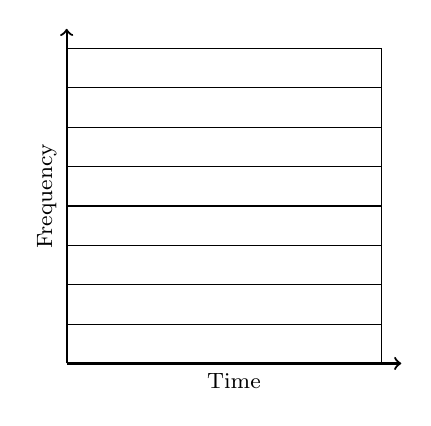
\begin{tikzpicture}
	\draw (0,0) -- (4,0);
	\draw (4,0) -- (4,-4);
	\path[thick, ->]  (0,-4) edge node[below] {\footnotesize Time} (4.25,-4)  ;
	\path[thick, ->] (0,-4) edge node[above, rotate=90] {\footnotesize Frequency} (0,.25)  ;
	
	\draw (0,-.5) -- (4,-.5);
	\draw (0,-1) -- (4,-1);
	\draw (0,-1.5) -- (4,-1.5);
	\draw (0,-2) -- (4,-2);
	\draw (0,-2.5) -- (4,-2.5);
	\draw (0,-3) -- (4,-3);
	\draw (0,-3.5) -- (4,-3.5);
	\end{tikzpicture}
	\caption{Fourier Transform}
\end{subfigure}

\medskip

\begin{subfigure}{.4\textwidth}
	\centering
		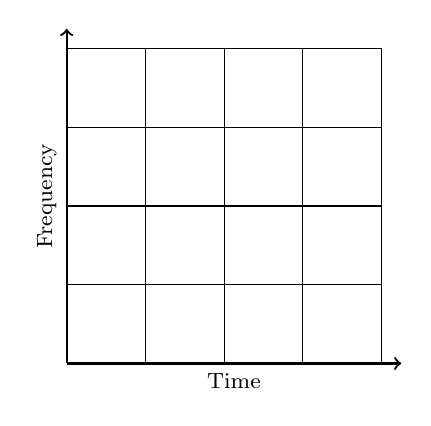
\begin{tikzpicture}
	
	\draw (0,0) -- (4,0);
	\draw (4,0) -- (4,-4);
	\path[thick, ->]  (0,-4) edge node[below] {\footnotesize Time} (4.25,-4)  ;
	\path[thick, ->] (0,-4) edge node[above, rotate=90] {\footnotesize Frequency} (0,.25)  ;
	
	\draw (1,0) -- (1,-4);
	\draw (0,-1) -- (4,-1);
	\draw (2,0) -- (2,-4);
	\draw (0,-2) -- (4,-2);
	\draw (3,0) -- (3,-4);
	\draw (0,-3) -- (4,-3);
	
	\end{tikzpicture}
	\caption{Short-Time Fourier Transform}
\end{subfigure}%
\begin{subfigure}{.4\textwidth}
	\centering
	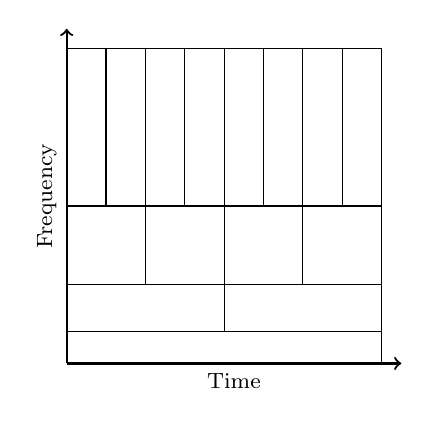
\begin{tikzpicture}
		\draw (0,0) -- (4,0);
		\draw (4,0) -- (4,-4);
		\path[thick, ->]  (0,-4) edge node[below] {\footnotesize Time} (4.25,-4)  ;
		\path[thick, ->] (0,-4) edge node[above, rotate=90] {\footnotesize Frequency} (0,.25)  ;
		\draw (0,-2) -- (4,-2);
		\draw (0,-3) -- (4,-3);
	
		\draw (0,-3.6) -- (4,-3.6);
		\draw (2,0) -- (2,-3.6);
	
		\draw[-] (1,0) -- (1,-3);
		\draw[-] (3,0) -- (3,-3);
	
		\draw[-] (.5,0) -- (.5,-2);
		\draw[-] (1.5,0) -- (1.5,-2);
	
		\draw[-] (2.5,0) -- (2.5,-2);
		\draw[-] (3.5,0) -- (3.5,-2);
	\end{tikzpicture}
	\caption{Wavelet Transform}
\end{subfigure}
\end{comment}
    \caption{Time—frequency resolution plane}
    \label{fig:time-frequency-plane}
\end{figure}

There are a wide variety of wavelets that serve different purposes like Morlet wavelet, Daubechies wavelet and many others.

\begin{figure}[H]
    \centering
    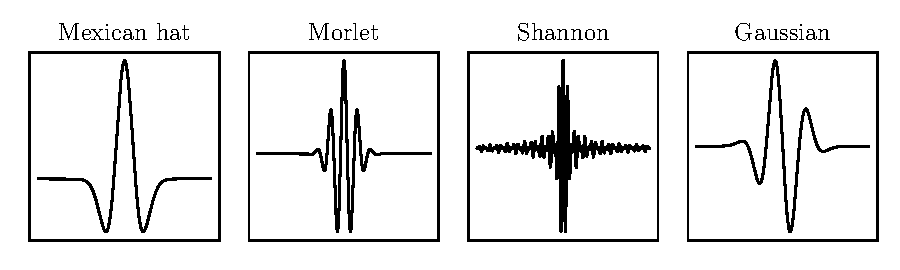
\includegraphics{figures/wavelets.pdf}
    \caption{Different types of wavelets}
    \label{fig:wavelets}
\end{figure}

\subsection{Continuous wavelet transform}
Mathematically, continuous wavelet transform is defined by equation \ref{equation:cwt}:

\begin{equation}
    CWT_x^\psi(\tau, s)=\frac{1}{\sqrt{|s|}}\int_{-\infty}^{\infty}x(t)\psi^* \left(\frac{t-\tau}{s}\right)dt
    \label{equation:cwt}
\end{equation}

Where $x(t)$ is the original signal, $\psi^*$ is a function called the \textbf{mother wavelet}; $s$ and $\tau$ are the \textbf{scale} and \textbf{translation} parameters respectively. The original signal is multiplied by the mother wavelet which is scaled using different scales then translated over the signal.

The output of \acrshort{cwt} is a scaleogram like the one in figure \ref{fig:scaleogram} which is a scaleogram (filled contour plot) of vibrations data snapshot of 25ms:

\begin{figure}[H]
    \centering
    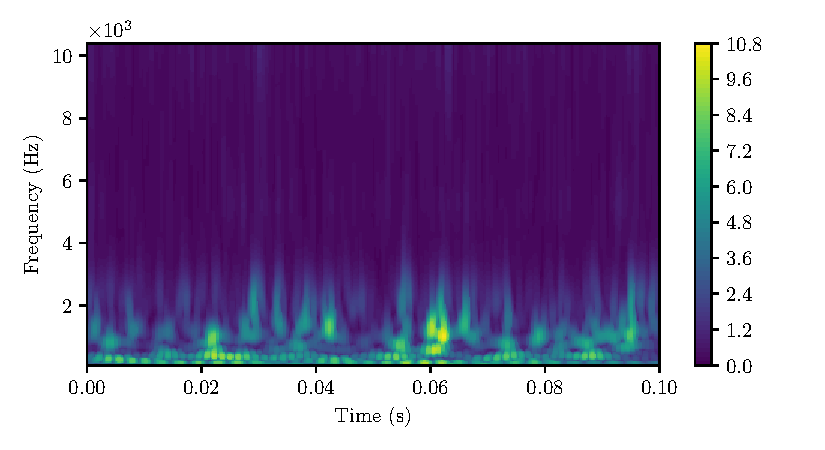
\includegraphics{figures/scaleogram.pdf}
    \caption{Scaleogram of vibration data snapshot}
    \label{fig:scaleogram}
\end{figure}

The x and y axes represent time and frequency respectively. Different colors indicate the power (i.e. amplitude) of each frequency (y-axis) during each instant of time (x-axis) which—unlike Fourier transform—provides information about the frequencies present in the signal and also the instances of time when these frequencies are present.

\subsection{Discrete wavelet transform}
In practical applicaions, discrete wavelet transform (DWT) is implemented as a filter bank where the signal is passed therough low- and high-pass filters to obtain \textbf{approximation} and \textbf{decomposition coefficients}. Figure \ref{fig:dwt} shows a DWT with 2 levels of decomposition which yields 2nd order approximation and decomposition coefficients:

\begin{figure}[H]
    \centering
    \begin{tikzpicture}[cell/.style={rectangle,draw, thick,align=center, minimum size=2em,inner sep=5pt}, input/.style={->}]

\node[cell] at (0,0) (xn) {$x[n]$};

\node[cell] at (-1.5,-1.5) (lpf1) {$LPF$};
\node[cell] at (1.5,-1.5) (hpf1){$HPF$};

\node[cell] at (-1.5,-3) (A1) {A1};
\node[cell, below = 1em of hpf1]  (D1) {D1};

\node[cell, below left = 2em of A1] (lpf2) {$LPF$};
\node[cell, below right = 2em of A1] (hpf2){$HPF$};

\node[cell, below = 1em of lpf2]  (A2) {A2};
\node[cell, below = 1em of hpf2]  (D2) {D2};

\draw[->, >=angle 60] (xn) -- ++(0,-1em) -- ++(0,-0.75em) -| (lpf1);
\draw[->, >=angle 60] (xn) -- ++(0,-1em) -- ++(0,-0.75em) -| (hpf1);

\draw[->, >=angle 60] (lpf1) -- (A1);
\draw[->, >=angle 60] (hpf1) -- (D1);

\draw[->, >=angle 60] (A1) -- ++(0,-1em) -- ++(0,-0.8em) -| (lpf2);
\draw[->, >=angle 60] (A1) -- ++(0,-1em) -- ++(0,-0.8em) -| (hpf2);

\draw[->, >=angle 60] (lpf2) -- (A2);
\draw[->, >=angle 60] (hpf2) -- (D2);

\node[] at (3,-0.9) (coord1) {};
\node[] at (3,-3.25) (coord2) {};

\end{tikzpicture}
    \caption{Discrete wavelet transform (DWT) as a filter bank}
    \label{fig:dwt}
\end{figure}

\begin{figure}[H]
    \centering
    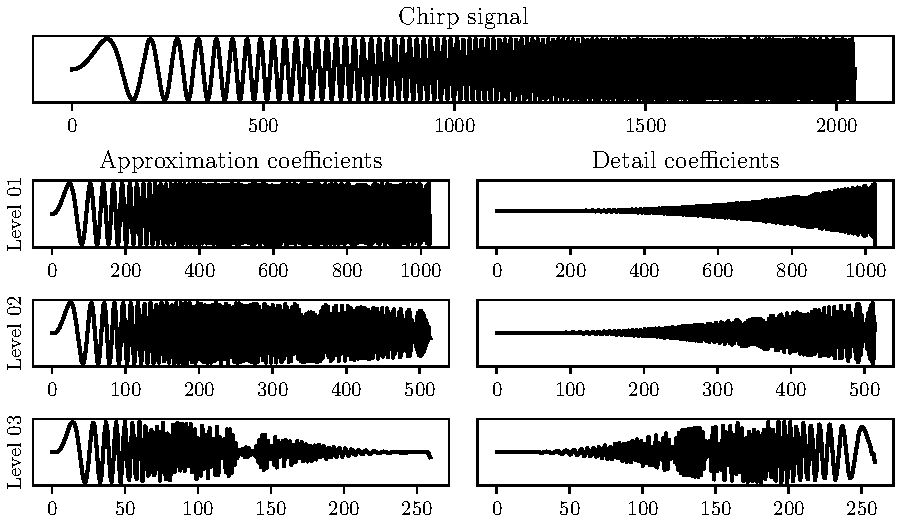
\includegraphics{figures/dwt_chirp.pdf}
    \caption{Level 3 signal decomposition using DWT}
    \label{fig:dwt-chirp-signal}
\end{figure}

DWT returns two sets of coefficients: \textbf{approximation coefficients} associated with the low pass filter and \textbf{detail coefficients} associated with the high pass filter of the DWT. By applying DWT again on the approximation coefficients the next level of decomposition can be obtained. At each level the original signal is downsampled by a factor of 2, this fact imposes a limitation on the possible number of decomposition levels for a given signal.

\section{Conclusion}
Vibration data are discrete signals sampled at a certain frequency in time. Although they hold so many valuable information about equipment performance, these information are usually not directly observable in the time domain. Digital signal processing techniques offer a way to gain more insights from raw vibration data by converting it to frequency or time–frequency domains where unusual frequency components can indicate development of certain degradation pattern. This chapter introduced several of these techniques like Fourier and Wavelet transforms. A following chapter will present the use of these techniques for extracting features that serve as an input for a neural network that can estimate the remaining useful life.
\end{comment}

